%1. Common problems and common technologies [+]
% - Text search +
% - Self Index +
% - Problems with self indexation +
% - Full text search with substrings +
%2. SA: overview, complexity, usage         [+]
%3. Radix: overview, complexity, usage      [+]
%4. Succinct data                           [+]
%5. CSA                                     [+]
%6. PSI                                     [+]
%7. Regenerating SA from PSI                [+]
%8. EF                                      [+]
%9. My CSA                                  []
%10.Complexity                              []

\textbf{Text retrieval}

Currently the Internet is updated with a large amount of data everyday.
That is why it is extremely important to organize search of necessary information in an \emph{effective} way.
In search within document indexing is applied.
\emph{Inverted index} is traditional for text indexing.
It is a data structure in which for each word in a document collection corresponding list
contains all the documents of a collection where this word is present.
While processing a multiple word request the intersection of lists is used,
that is corresponded to each word in a query.

\textbf{Problems of traditional approaches}

Some cases take place in practice where it is impossible to use
traditional full-text search by words \cite{bast2013efficient}.
A search model in which the task is to find orthographically close words (\emph{fuzzy search}),
that is used for spelling correction in numerous text editors,
does not allow one to solve the problem using full-text search.
The same applies to different systems where \emph{pattern matching} is used \cite{bai2018adaptive}.
Another example of texts where it is difficult to apply traditional search method
are several eastern languages.
In these languages words are not separated by spaces that makes \emph{inverted index} difficult to use.
Finally large texts combined from alphabet with a small amount of symbols
can be attributed to <<inconvenient>> texts.
A typical example of these texts is DNA and protein structure code.
This text is not separated on words that is a key issue in using \emph{inverted index}.

To solve these problems it is necessary to perform substring search.
Existing methods (prefix tree, suffix array) take too much space therefore they are not effective.
For example, prefix tree that contains \emph{n} words with $C$ average number of symbols in a word
takes $O(n \cdot C)$ memory \cite{aho1975efficient}.
Let's take a greater look at suffix array as one of the most popular textual information indexation methods.

\textbf{Full-text search using suffix array}

Suffix array is a data structure used in full-text search that allows one to perform
substring search in a text consisting of \emph{n} symbols in $O(\log{}n)$ \cite{manber1993suffix}.
To store \emph{n} words in suffix array it is necessary to use $O(n \log{}n)$ of memory.
For instance, $2^{32}$ ASCII-text requires $2^{32} \cdot 8 = 32$ GB memory space.
For this text suffix array must contain 32 bit elements.
Therefore, suffix array size reaches $2^{32} \cdot 32 = 128$ GB memory space that is
4 times greater than the initial text size.

Suffix array is a sorted in a lexicographic order sequence of suffixes.
In order to better understand the structure of suffix array, consider this data structure
using as an example word <<mississippi>>:
\\(0) mississippi
\\(1) ississippi
\\(2) ssissippi
\\(3) sissippi
\\(4) issippi
\\(5) ssippi
\\(6) sippi
\\(7) ippi
\\(8) ppi
\\(9) pi
\\(10) i

Suffix array consisting of these suffixes would be presented as:

10 7 4 1 0 9 8 6 3 5 2

Usually the end of document is indicated by a special symbol that is not included in
the alphabet of a text stored in the array.
As a delimiter in this paper dollar symbol \$ has been chosen.
Modern approaches to suffix array construction allows one to  build data structure in $O(n)$.

\textbf{Radix tree}

% Picture By Claudio Rocchini - Own work, CC BY 2.5, https://commons.wikimedia.org/w/index.php?curid=2118795

\begin{wrapfigure}{r}{0.25\textwidth} %this figure will be at the right
 \centering
 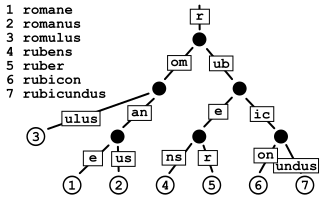
\includegraphics[width=0.45\textwidth]{PatriciaTrie}
 \caption{Radix tree example}
\end{wrapfigure}

Radix tree is a compressed prefix tree. In its turn, prefix tree is a data structure
that represents the intreface of associative array and allows one to store values in key-value pairs.
In this paper the string is chosen as a key, and in a contrary to regular trees,
the edges can contain either one element (symbol), or a sequence of elements (string).

Radix tree is commonly used in Linux kernel to bind a pointer with a long integer key \cite{Linux2018}.
This data structure is effective from the perspective of a search speed and data storage.
At the same time, Radix tree is used in IP-addressing because it is extremely useful for
hierarchical IP-addressing structure \cite{Radix2019} storage.

Let's take a detailed look at radix tree characteristics. Let us assume that it is required
to store keys the size of \emph{k} storing \emph{n} elements at the tree. Then insertion of an element,
search and removal take $O(k)$ operations \cite{leis2013adaptive}.

For many dictionary search requests radix tree can be faster and more effective than hash tables.
Despite the fact that often the complexity of search in a hash table is considered to be $O(1)$,
the necessity for the initial caching of input data is ignored in this assumption.
It takes $O(k)$ operations where \emph{k} is the length of input string.
Radix tree performs the search in $O(k)$, without initial data caching and has greater
cache localization characteristics.
It also preserves the order allowing one to perform an ordered scan,
get min / max values, scan over common prefix etc.

Because of all these advantages, radix tree is widely used in a Redis data base, program
products of HashiCorp, such as Terraform, Consul, Vault, Nomad etc \cite{Redis2018},
that is of additional interest for studying it on textual data and comparison with suffix array.

\textbf{Succinct data representation}

One of the most important problems of this research is
a program implementation of succinct index storage for suffix array.
That is why it is important to understand what data can be considered succinct.

There are several degrees of information compression.
Let us assume that the storage of a piece of data takes \emph{Z} bit.
Succinct data structures take \(Z + o(Z)\) bit, implicit -- \(Z + o(1)\) bit and
compact -- \(O(Z)\) bit \cite{huo2014practical}. In this paper it is proposed to
compress suffix array in succinct data representation.
Thus, the size of array is only a little bit greater than the size of initial text.

\textbf{$\Psi$-array}

An important part in a theory of succinct index representation is taken by an intermediate $\psi$-array.
A characteristic feature of all the compression algorithms of a compressed suffix array (CSA) is 
that not the index itself is compressed but it's representation as a $\psi$-array.
Auxiliary array can be obtained from suffix array by the following index manipulations.
Let us consider a $\psi$-array construction by the example of a familiar string \textbf{mississippi\$}:
\\ \textbf{Text}:\,\,\,\,\,\,\,\,\,\,\,\,\,\,\,\,\,\,\,\,\,\,\,\,
m \,i \,\,\,\,s \,\,\,s \,\,\,\,i \,\,\,\,s \,\,\,s \,\,i \,\,p \,\,p \,\,i \,\,\,\,\$
\\ \textbf{Offset}:\,\,\,\,\,\,\,\,\,\,\,\,\,\,\,\,\,\,\,\, 0 \,\,1
\,\,\,\,2 \,\,3 \,\,\,4 \,\,\,5 \,\,6 \,7 \,\,8 \,\,9 \,10 11
\\ \textbf{Suffix Array}:   11 10 \,7 \,\,4 \,\,\,1 \,\,\,0 \,\,9 \,8 \,\,6 \,\,3 \,\,5 \,\,2
\\ \textbf{$\Psi$ -array}: \,\,\,\,\,\,\,\,\,\,\,\,\$ \,\,\,0 \,\,\,\,7
10 \,\,11 4 \,\,1 \,6 \,\,2 \,\,3 \,\,8 \,\,9

Let us call the largest suffix of a substring except for the initial string as a successor.
Therefore, for substring issippi\$ successor is ssippi\$.
$\Psi$-array points out to a successor for every chosen suffix.
As an example consider $SA[7] = 8$. It's successor is a position in a suffix array that contains $8 + 1 = 9$.
Thus, $\psi[7] = 6$. The main relation between a $\psi$-array and suffix array:
\begin{equation}\label{sa:1}
SA[i] = SA[\psi[i]] - 1
\end{equation}
It is necessary to emphasize that $\Psi[0] = \$$, because there is no successor
for the first element in a suffix array.
However, $SA[5]$ is reffered to 0 index, that is the whole string overall.
In other words, the element of suffix array is reffered to the beginning of the text,
that is no other suffix can have it as a child.
There is no element equal to 5 in a $\psi$-array, respectively.

\textbf{Suffix array reconstruction from a $\psi$-array}

There is an opportunity to reconstruct the initial suffix array by generated $\psi$-array
with operations that are reversive to those that were present in the last paragraph.
Let us have a better look at the specific features of this algorithm.

First of all, it is necessary to find the index of the element of suffix array
that has not been present in the $\psi$-array.
In our example it is equal to 5. From the discussions above, it can be seen that $SA[5] = 0$.
Thus, one element of an initial suffix array was reconstructed. From the formula \ref{sa:1} for $i = 5$ follows:

\[SA[5] = SA[\psi[5]] - 1\]
\[0 = SA[4] - 1\]
\[SA[4] = 1\]

Another element of a suffix array is reconstructed!
This way the whole remaining sequence can be reconstructed.
Time taking to find the first element is equal to \(O(n)\) operations.
There are several improvements of the search speed of a certain elements in a suffix array
that require additional data structures storing suffix array values at every \(\log n\) step \cite{andersensimple}.
This approach goes beyond this paper, because the main problem of it is to find the best index compression.

\textbf{$\Psi$-array compression}

Let us have a detailed look at $\psi$-array:
\\ \textbf{Text}:\,\,\,\,\,\,\,\,\,\,\,\,\,\,\,\,\,\,\,\,\,\,\,\,
m \,i \,\,\,\,s \,\,\,s \,\,\,\,i \,\,\,\,s \,\,\,s \,\,i \,\,p \,\,p \,\,i \,\,\,\,\$
\\ \textbf{Offset}:\,\,\,\,\,\,\,\,\,\,\,\,\,\,\,\,\,\,\,\, 0 \,\,1 \,\,\,\,2
\,\,3 \,\,\,4 \,\,\,5 \,\,6 \,7 \,\,8 \,\,9 \,10 11
\\ \textbf{Suffix Array}:   11 10 \,7 \,\,4 \,\,\,1 \,\,\,0 \,\,9 \,8 \,\,6
\,\,3 \,\,5 \,\,2
\\ \textbf{$\Psi$ -array}: \,\,\,\,\,\,\,\,\,\,\,\,\$ \,\,\,0 \,\,\,\,7 10 \,\,11 4
\,\,1 \,6 \,\,2 \,\,3 \,\,8 \,\,9

Sorted suffix array looks like that:
\\ (0) \,\,\,\$
\\ (1) \,\,\,i\$
\\ (2) \,\,\,ippi\$
\\ (3) \,\,\,issippi\$
\\ (4) \,\,\,ississippi\$
\\ (5) \,\,\,mississippi\$
\\ (6) \,\,\,pi\$
\\ (7) \,\,\,ppi\$
\\ (8) \,\,\,sippi\$
\\ (9) \,\,\,sissippi\$
\\ (10) ssippi\$
\\ (11) ssissippi\$

It is worth mentioning the structure of it: it contains a set of adjusting indices.
Let us consider the ascending sequence 2, 3, 8, 9.

$SA[2] = 7$, $T[7] = i$.
$SA[3] = 4$, $T[4] = i$.

It is noteworthy that $SA[6] = 9$, $T[9] = p$.
Thus the alternation of the index from increase to decrease corresponds to
the switch of symbols from \emph{i} to \emph{p}.

\begin{theorem}
 \label{lemma:1}
 Two consequent elements of a $\psi$-array are ascending if corresponding suffixes that they are referred to
 start from the same symbol.
\end{theorem}

\begin{proof}
    By construction, suffix array is a set of indices in the initial text,
    sorted in lexicographic order. It means that $T[SA[i]] < T[SA[i + 1]]$
    $\forall i \in [0, n).$ These two suffixes have common first symbol.
    That is why they are different in the following elements, e.g. in the second one:
    $T[SA[i] + 1] < T[SA[i + 1] + 1].$

    $\Psi$-array is reffered to a successor of a given suffix: $T[SA[\psi[i]]] < T[SA[i] + 1].$
    Because $T[SA[i]]$ and $T[SA[i + 1]]$ have the same first symbol, their successors are ordered.
    If $T[SA[\psi[i]]] < T[SA[\psi[i + 1]]]$, then because of orderliness the index in suffix array
    for the first one should precede the index for the second one. Therefore, indices (values of $\psi$-array)
    should be ordered if suffixes have a common first symbol.
\end{proof}

Ascending sequences of non-negative integer numbers are compressible \cite{andersensimple}.
The easiest way to store these sequences is a bitmap.
However, this method does not allow one to have a random access to the elements.
Let us consider in detailes a more advanced algorithm of succinct data representation.

\textbf{Elias--Fano Encoding}

Compression via Elias--Fano method \cite{pibiri2014dynamic}
allows one to represent monotonically increasing sequences
of non-negative integer numbers in the form of bit vectors. This approach makes possible to
store a non-decreasing sequence of $n$ integer values the size of $[0, m)$,
taking $2n + n[\log m/n]$ bit, allowing access to the $i$-th element in $O(1)$.
Comparing the size of data structure with a minimal possible space in a memory
from the theory of information point of view, Elias--Fano coding is a succinct index.

\begin{figure}[t]
 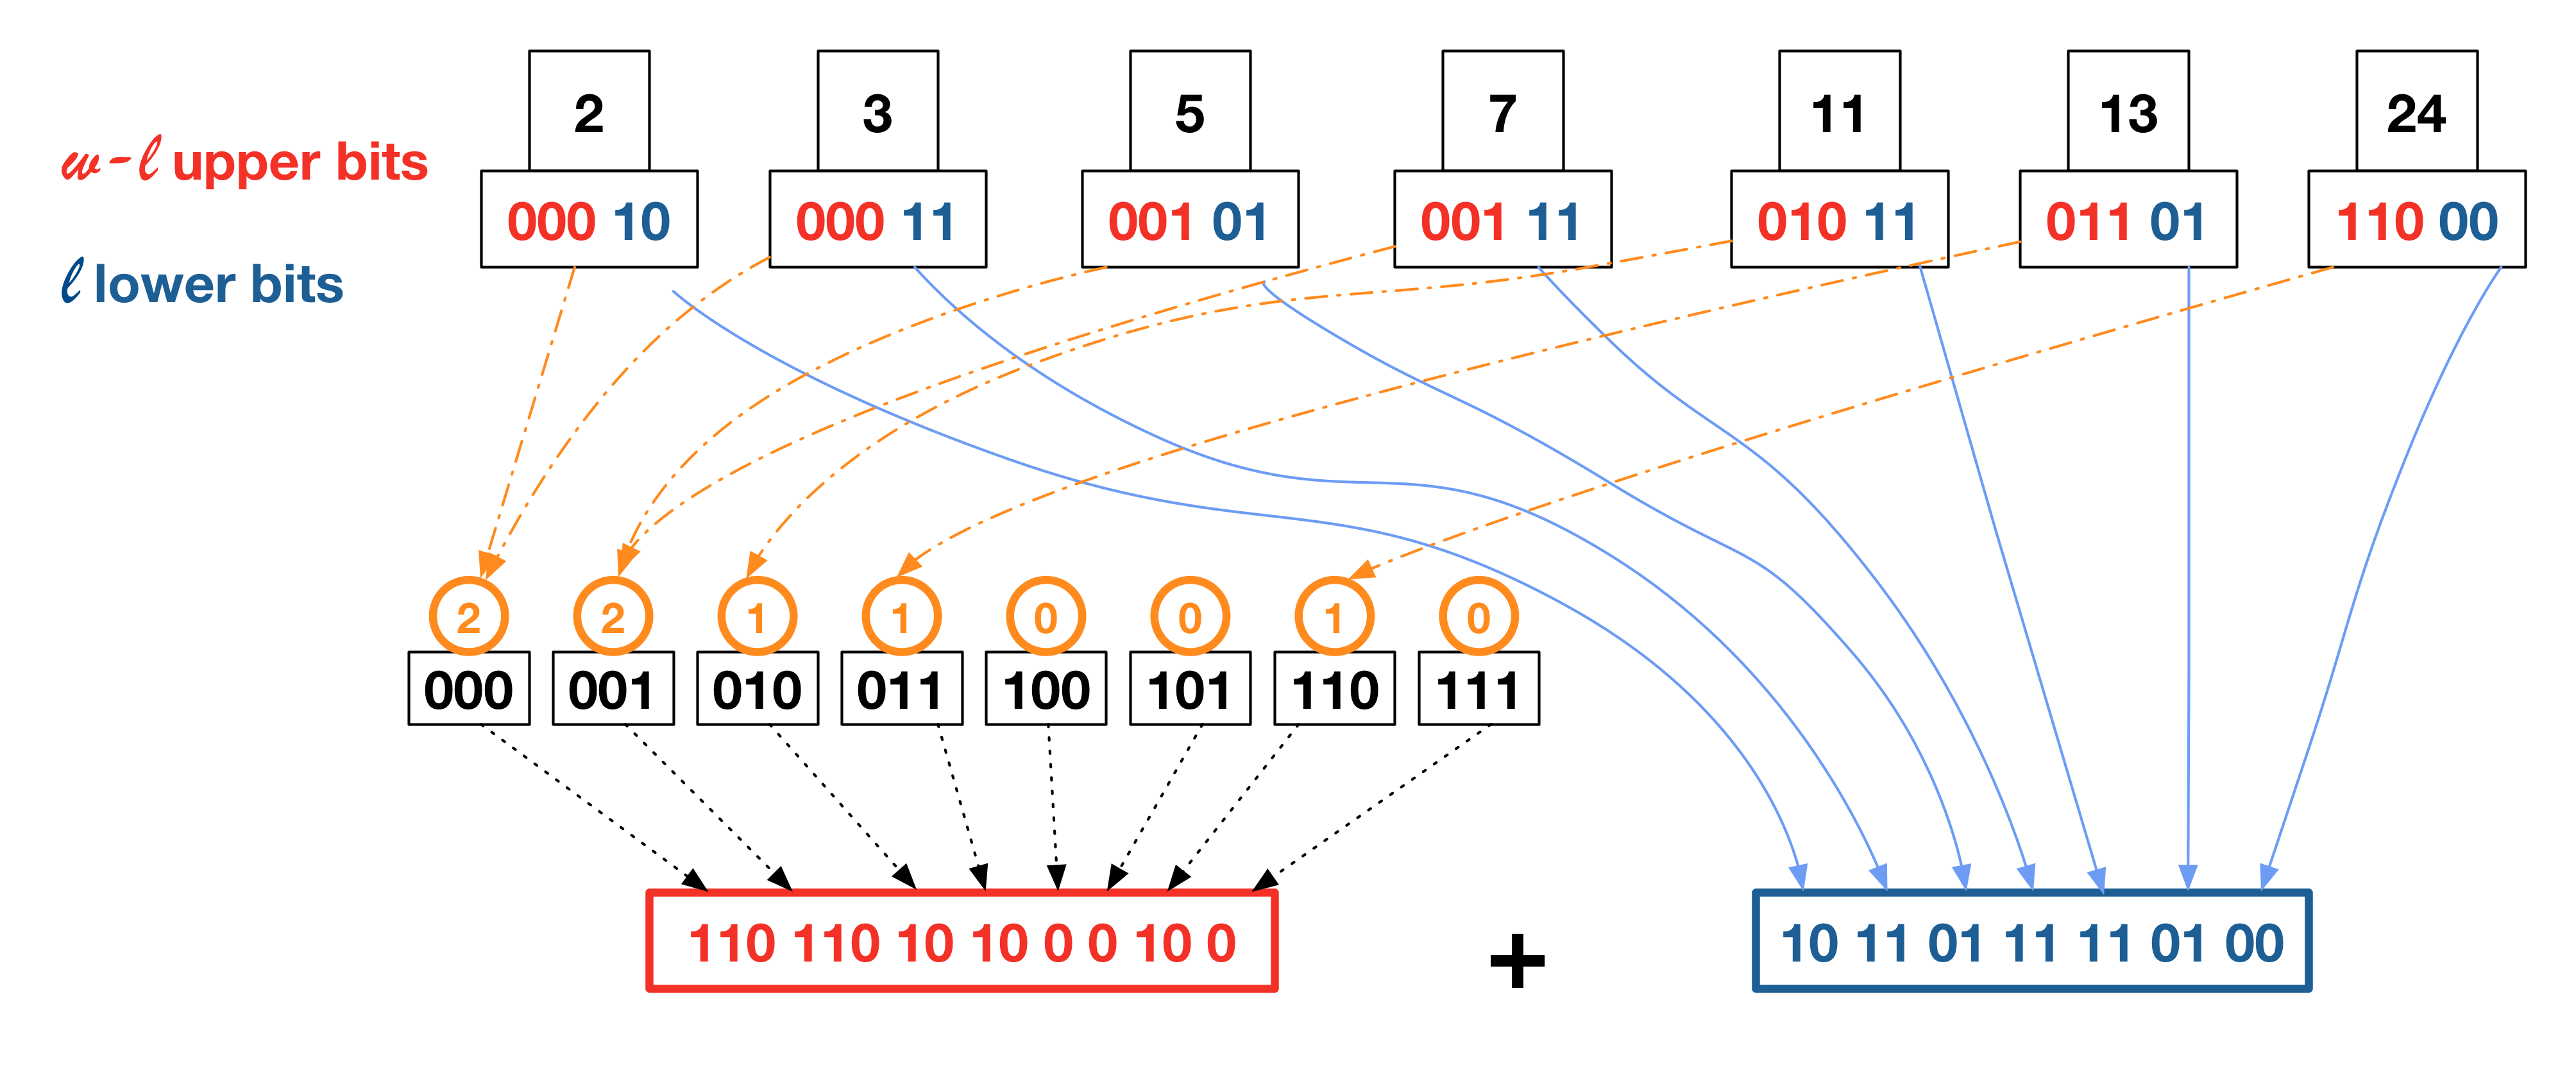
\includegraphics[width=12cm]{Elias-Fano}
 \caption{Example of the code construction for Elias-Fano}
 \centering
 \label{fig:EF}
\end{figure}

In the beginning each number from the sequence is encoded by $\log m$ bits of data.
Binary elements representation is devided by two parts: upper one, containing
first $\log n$ bit, and lower one with the remaining $\log m - \log n = \log m / n$ bit.
The union of lower bits takes $n \log m$ bit. Upper bits are a set of 
$n + m / 2^{\log m/n}$ bit \cite{antonio2018integers}.
Starting from an empty bit vector, we add 0 to this part as a stop-bit
for each possible value represented by the bits of an upper part.
For each actually present value 1 is added, setting it before the corresponding stop-bit.

Let us consider as an example a sorted sequence {2,3,5,7,11,13,24}.
The figure \ref{fig:EF} shows a coding scheme. The largest number in the universe is 24.
Therefore for the representation of each element it is necessary to allocate 5 bits per element.
Then the binary representation is separated into two parts: upper and lower one.
Starting from the conditions described before, let us choose 3 bits for an upper part and 2 bits for a lower one.
Overall there are 7 elements in a sequence. Let us consider number 2.
For it we have $2 = 0b00010$ and 000 as an upper part and 10 as a lower part correspondingly.
Repeating this process, a set of upper and lower parts will be obtained for each element.
Then these parts are combined together. For upper parts there are $2^3$ variants of sets of values.
With each of these numbers a counter is associated that increases by one if a number from the sequence
has the same upper part. So for 2 the set 000 is incremented. A number $3 = 0b00011$ with 000 upper part
goes to the same set. For a number $5 = 0b00101$ with 001 upper part, the set 001 is incremented and so on.
Finally, the unary coding is performed, adding as many 1s in a counter representation as it is a value of
each counter after which there is a 0-bite. The resulting Elias-Fano encoding is a union of obtained
upper and lower parts.

\textbf{Data resconstruction from the Elias--Fano code}

For an initial reconstruction of a monotonically non ascending sequence of numbers it is necessary to
desing an operation with an access to the $i$-th element of a sequence, $i \in [0, n)$.
To access the lower part it is possible to get corresponding bits because the length of a vector for
the element storage is known.
To get the upper part it is necessary to perform a \emph{select} operation. \emph{Select($i$)}
operation allows one to get a postion of the $i$-th bit set to 1 in a bitvector.
This operation takes $O(1)$ time that provides a random access to an element
of the sequence without a complete decoding of the whole sequence overall \cite{farina2009rank}.
